\documentclass{mproj}
\usepackage{graphicx}

\usepackage{url}
\usepackage{fancyvrb}
\usepackage[final]{pdfpages}
\usepackage{times}
\usepackage{pdfpages}
\usepackage{amsmath}
\usepackage{float}

% for alternative page numbering use the following package
% and see documentation for commands
%\usepackage{fancyheadings}


% other potentially useful packages
%\uspackage{amssymb,amsmath}
%\usepackage{url}
%\usepackage{fancyvrb}
%\usepackage[final]{pdfpages}

\begin{document}

%%%%%%%%%%%%%%%%%%%%%%%%%%%%%%%%%%%%%%%%%%%%%%%%%%%%%%%%%%%%%%%%%%%
\title{Energy Efficient Knowledge Distribution in Wireless Sensor Networks for Query Analytics}
\author{Kurt Portelli}
\date{\today}
\maketitle
%%%%%%%%%%%%%%%%%%%%%%%%%%%%%%%%%%%%%%%%%%%%%%%%%%%%%%%%%%%%%%%%%%%

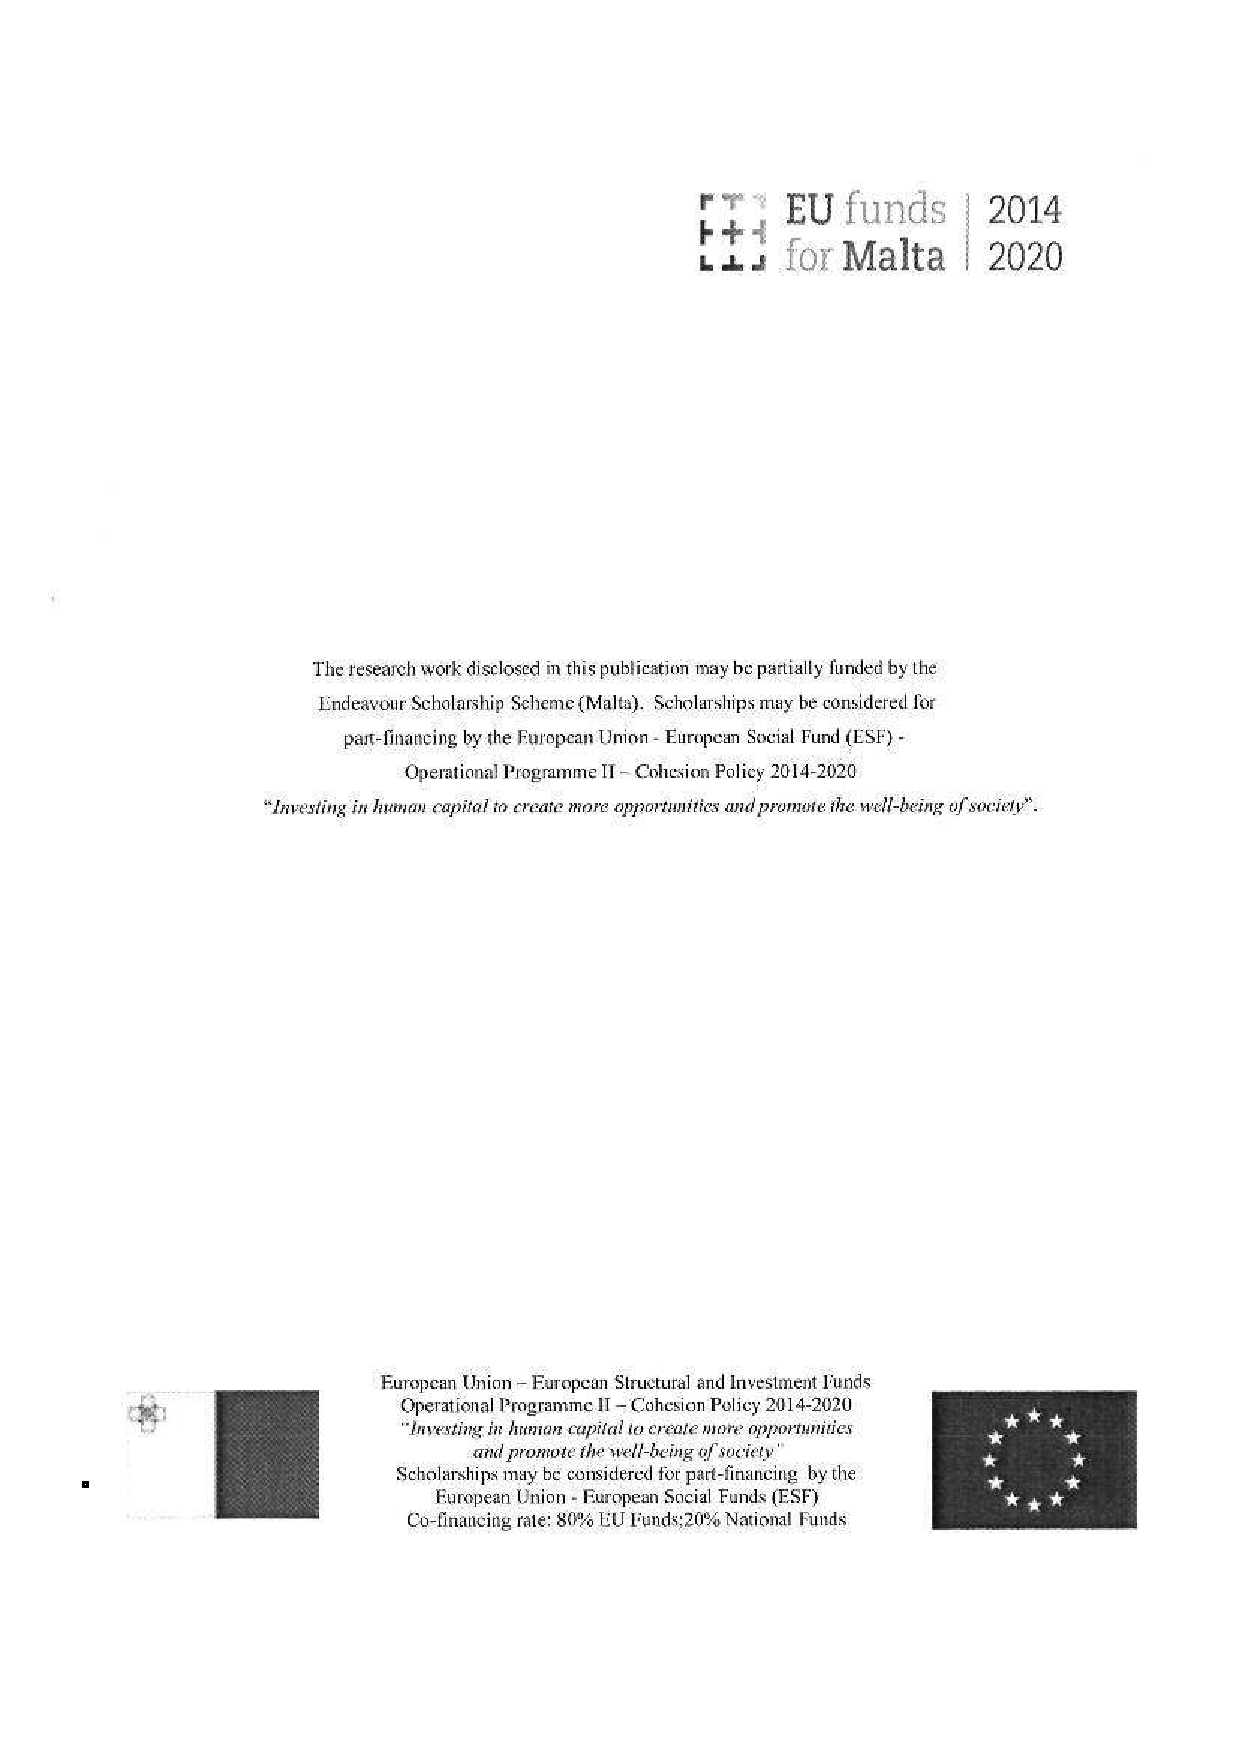
\includepdf[pages={1}]{ENDEAVOUR-Acknowledgement.pdf}

%%%%%%%%%%%%%%%%%%%%%%%%%%%%%%%%%%%%%%%%%%%%%%%%%%%%%%%%%%%%%%%%%%%
\begin{abstract}


\end{abstract}
%%%%%%%%%%%%%%%%%%%%%%%%%%%%%%%%%%%%%%%%%%%%%%%%%%%%%%%%%%%%%%%%%%%

%%%%%%%%%%%%%%%%%%%%%%%%%%%%%%%%%%%%%%%%%%%%%%%%%%%%%%%%%%%%%%%%%%%
\educationalconsent

%%%%%%%%%%%%%%%%%%%%%%%%%%%%%%%%%%%%%%%%%%%%%%%%%%%%%%%%%%%%%%%%%%%

\newpage
%%%%%%%%%%%%%%%%%%%%%%%%%%%%%%%%%%%%%%%%%%%%%%%%%%%%%%%%%%%%%%%%%%%
\section*{Acknowledgements}
I wish to express my sincere gratitude to Dr. Christos Anagnostopoulos for his guidance and expert advice throughout all the various stages of this project. Apart from that I am also thankful to him for making me appreciate even more the subject of data science and machine learning.

Furthermore, I would like to thank my family for all their continuous support in this first year living abroad. 


%%%%%%%%%%%%%%%%%%%%%%%%%%%%%%%%%%%%%%%%%%%%%%%%%%%%%%%%%%%%%%%%%%%
\tableofcontents
%%%%%%%%%%%%%%%%%%%%%%%%%%%%%%%%%%%%%%%%%%%%%%%%%%%%%%%%%%%%%%%%%%%


\chapter{Introduction}\label{intro}
The Internet of Things (IoT) is a rapidly growing area, with it more data is being stored and made accessible which previously has never even been thought possible. IoT is composed of billions of devices that can gather, share information and sometimes even capable of performing operations on this information. IoT devices are physical objects connected with the internet able to share information. This can include anything ranging from smartphones to Radio Frequency Identification (RFID) tags found in everyday products. As more data is made available for anything imaginable that affects our daily lives, opportunities arise for applications that extract this information and make use of it.
EXAMPLE SMARTGRID AND REFERENCE. Making all this information useful is very challenging as it needs to be collected, transferred, stored and made accessible. 

In a naive system all these devices generate massive amounts of data which is periodically sent to central node with more computing resources. This in turn, might restructure the data more effectively to be sent to another node or make it available for querying. All this network transfer drains power and as the network size increases this effect is emphasized even more. This has created a need and opportunity for machine and statistical learning algorithms.\cite{LargeScaleOnlineLearning} According to L.Bottou et al.\cite{LargeScaleOnlineLearning} these technological improvements have outrun the exponential evolution of computing power. Thus, we must rely more on on-line learning algorithms to process these large amounts of data with comparatively less computing power.

The vision of IoT is to allow any device to be continuously connected sharing its knowledge about the surroundings. Machine learning then uses this stream of data to deduce results, infer new knowledge, reason about contextual events or make assumptions. The possibilities for such systems are endless, taking, for instance, the case of thermometers in rooms next to each other and based on previous information the temperature of various rooms can be predicted based on the temperature of adjacent ones.

\section{Problem Synopsis}


\section{Project Aims}

\section{Document Outline}

\chapter{Preliminaries}
In this chapter, we present an overview of the concepts and base principles we mention and make use of in our work. We develop a system which deals with a continuous data stream and thus, has to use specialized algorithms which treat each data item individually without storing past data items. Various algorithms are used which extract knowledge from each individual sensor by minimizing loss and then quantize the input.

\section{On-line Algorithms}
According to M.Karp \cite{Karp} an on-line algorithms is one which receives a sequence of requests and performs an immediate action to each request. These are useful in situations where decisions must be made without any future knowledge. Their effectiveness is measured by the comparing them with their off-line (batch) counterparts. In this dissertation we make use of well known common techniques already proven to work.

\subsection{K-Means}
The K-means algorithm attempts to find K representatives (centroids) of a data set in such a way as to best represent the data. \cite{onlinekmeans} Although it is algorithmically simple, it still manages to be relatively robust and give close to optimal results on a wide range of data sets. Its disadvantage is that one has to predefine K. Furthermore, the initial K centroids chosen have a drastic effect upon the clusters chosen. The first k inputs initialize the codebook vectors (centroids) $m_j,j=1,...,k$. The rest of the inputs $x^t \in X$ are used for the update function.
\begin{equation}
\label{eq:chooseCluster}
i \longleftarrow arg min_j \parallel x^t - m_j \parallel
\end{equation}
\begin{equation}
\label{eq:updateCluster}
m_i \longleftarrow m_i + \eta (x^t - m_i)
\end{equation}
Equation \ref{eq:chooseCluster} finds the closest centroid to the input. Then the closest centroid is updated as shown in equation \ref{eq:updateCluster} depending on the learning rate defined by $\eta$. A large $\eta$ enhances accuracy but makes $m_i$ oscillate. Therefore to reach convergence one needs to use a small or decaying $\eta$.

\subsection{Adaptive Resonance Theory (ART)}
ART\cite{art} is another unsupervised learning algorithm similar to k-means. It does not require the number of clusters to be predefined before hand. Instead one has to define \textit{vigilance} which represents the degree of similarity between points. An data item $x^t \in X$ is a member of a cluster $m_j$ only if the distance between them is less than vigilance. Similar to the K=means procedure, once $m_j$ is chosen, equation {eq:updateCluster} is used to update the centroid. If no centroid satisfies this constraint, then a new cluster is created. This allows a better flexibility but has the disadvantage of creating an infeasible and unpredictable amount of clusters in certain situations.

\subsection{Linear Regression}
Once it is proven that there is a statistically significant correlation between two variables, linear regression allows us to make predictions about one variable based only on the other variable. The relationship between these two values must be linear, else this technique would not be able to model the data accurately.

To perform this supervised learning we must first start by defining the hypothesis example the linear function \ref{eq:hypothesis}.
\begin{equation}
\label{eq:hypothesis}
h_\theta(x) = \theta_0 + \theta_1x_1 + \theta_2x_2
\end{equation}
The $\theta_i$'s represent the weights of the linear function, thus, determining the mapping between X and Y. Let $x_0=1$, we then rewrite equation \ref{eq:hypothesis} to a more compact form represented by equation \ref{eq:hypothesisShort}.
\begin{equation}
\label{eq:hypothesisShort}
h(x) = \sum_{i=0}^{n} \theta_ix_i = \theta^Tx
\end{equation}
For this hypothesis to be useful, the $\theta$ parameters need to be trained to fit a particular dataset. Conceptually the closest $h(x)$ is to Y, the better we are at representing the data. Thus, we define the cost function equation \ref{eq:costFunction} which measures the total discrepancy for each input $x^{(i)}$ with output $y^{(i)}$.
\begin{equation}
\label{eq:costFunction}
J(\theta) = \frac{1}{2}\sum_{i=1}^{m}( h_\theta(x^{(i)})-y^{(i)})^2
\end{equation}
Naturally, we would like to choose a theta which minimizes the error. One such technique which does this is the gradient descent rule. It calculates the gradient of the error and takes a step proportional to the negative gradient. To achieve this we need to use the partial derivative of equation \ref{eq:costFunction}. For all $\theta$ the update rule then becomes equation \ref{eq:updateDerivative}. This update rule is called least mean squares (LMS) and it has a very interesting property. The magnitude of the update is proportional the the error. This means that the greater the error, the steeper the descent towards the minima.  After completing the derivative we are left with the complete equation \ref{eq:batchUpdate}. This has to be repeated for each $\theta$ until convergence. Meaning until we reach the best possible theta values.
\begin{equation}
\label{eq:updateDerivative}
\theta_j := \theta_j - \alpha\frac{\partial}{\partial\theta_j}J(\theta)
\end{equation}
\begin{equation}
\label{eq:batchUpdate}
\text{Repeat until convergence: (For each j) }
\theta_j := \theta_j - \alpha\sum_{i=1}^{m}(y^{(i)}-h_\theta(x^{(i)}))x_j^{(i)}
\end{equation}
One might argue that with this iterative approach we might get stuck at a local minima instead of finding the optimal minima. In this particular scenario J is a convex quadratic function, meaning it has only one minima. Thus, gradient descent will always converge at the global minima assuming $\alpha$ is not too large.

\subsubsection{Multivariate Stochastic Gradient Descent}
The previous algorithm is called batch gradient descent as for each update step it uses all all the training set. This would not be feasible to compute especially as the dataset size increases. Another issue would be that previous data items have to be stored, and this is not always possible. In fact we will be using the more lightweight and on-line version called stochastic gradient descent. In batch gradient descent we go through all the data set for a single update step while when using equation \ref{eq:stochUpdate} we start making progress right away. We use this update rule for each new training item we encounter. This in fact has the tendency of getting close to $\theta$ much faster than batch gradient descent, however it may never converge and instead keep oscillating around the minimum. The reason it is called multivariate is that we will be using multiple inputs (more than one $x$) to get $y$.

\begin{equation}
\label{eq:stochUpdate}
\text{(For each j) }\theta_j := \theta_j + \alpha(y^{(i)}-h_\theta(x^{(i)}))x_j^{(i)}
\end{equation}

\subsection{Mean and Variance}

\section{Probability Distribution Function}

\section{Normalization}
We use the standard score \cite{normalization} to normalize the dataset. This is done by subtracting each item $x$ by the mean and then dividing it by the standard deviation of the dataset as shown in equation \ref{eq:standardScore}. Performing this normalization allows us to better understand the results as it gives a meaning to a raw value. Figure \ref{fig:zscore} demonstrates the distribution of $z$, a negative value means that x was less than the mean. Furthermore, the magnitude of this value represents the distance from the mean in terms of standard deviation.
\begin{equation}
\label{eq:standardScore}
z= \frac{x - \mu}{\sigma}
\end{equation}
\begin{figure}[H]
\caption{Standard score normalization \cite{normalization}}
\label{fig:zscore}
\centerline{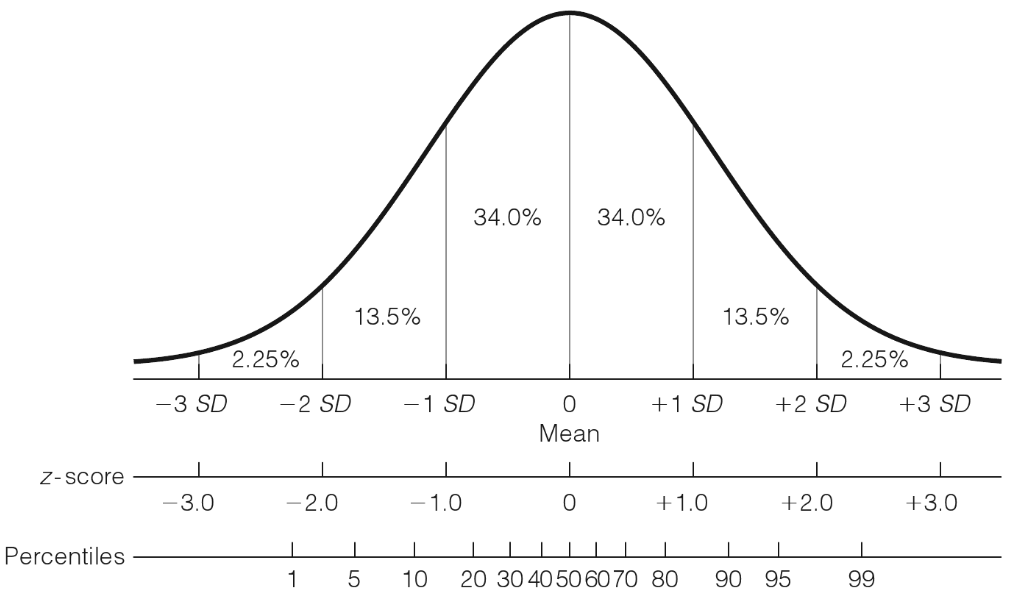
\includegraphics[scale=0.4]{zscore}}
\end{figure}

\section{K Nearest Neighbours (KNN)}
KNN \cite{knn} is a straightforward classification technique, in which given an input it is able to classify it to certain class. As the name implies it takes the closest K neighbours and depending on the majority of their classes it determines the class of the input. Figure \ref{fig:knn} demonstrates KNN ($K=3$) while classifying X using a data set containing 3 different classes. In this case input X is classified as Red due to the fact that the majority of its 3 closest neighbours are Red.
\begin{figure}[H]
\caption{At KNN=3, Input X is classified as Red}
\label{fig:knn}
\centerline{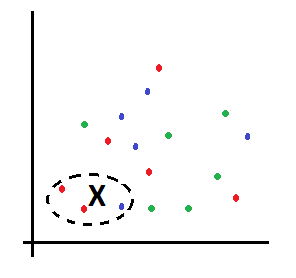
\includegraphics[scale=1]{knn}}
\end{figure}

\chapter{Literature Review}

\chapter{Contributions}

\section{Network Efficiency}

\section{Ensemble Learning}

\section{Optimal Stopping}

\chapter{Design and Implementation}

\section{Network Architecture}

\section{Query Analytics}

\chapter{Evaluation and Case Study}

\section{Data Set}

\section{Error Allowance vs Messages Sent}

\section{Probability Distribution Functions}

\section{Query Validation}

\chapter{Conclusion}\label{conclusion}

\section{Achievements}

\section{Future Work}

\section{Final Remarks}

\appendix % first appendix

\chapter{First appendix}

\section{Section of first appendix}

\chapter{Second appendix}

\bibliographystyle{plain}
\bibliography{mproj}
\end{document}
